\documentclass[tikz,border=6pt]{standalone}
\usepackage{pgfplots}
\pgfplotsset{compat=1.18}
\definecolor{blue}{RGB}{37,99,235}
\definecolor{violet}{RGB}{124,58,237}
\definecolor{grayx}{RGB}{100,116,139}
\begin{document}
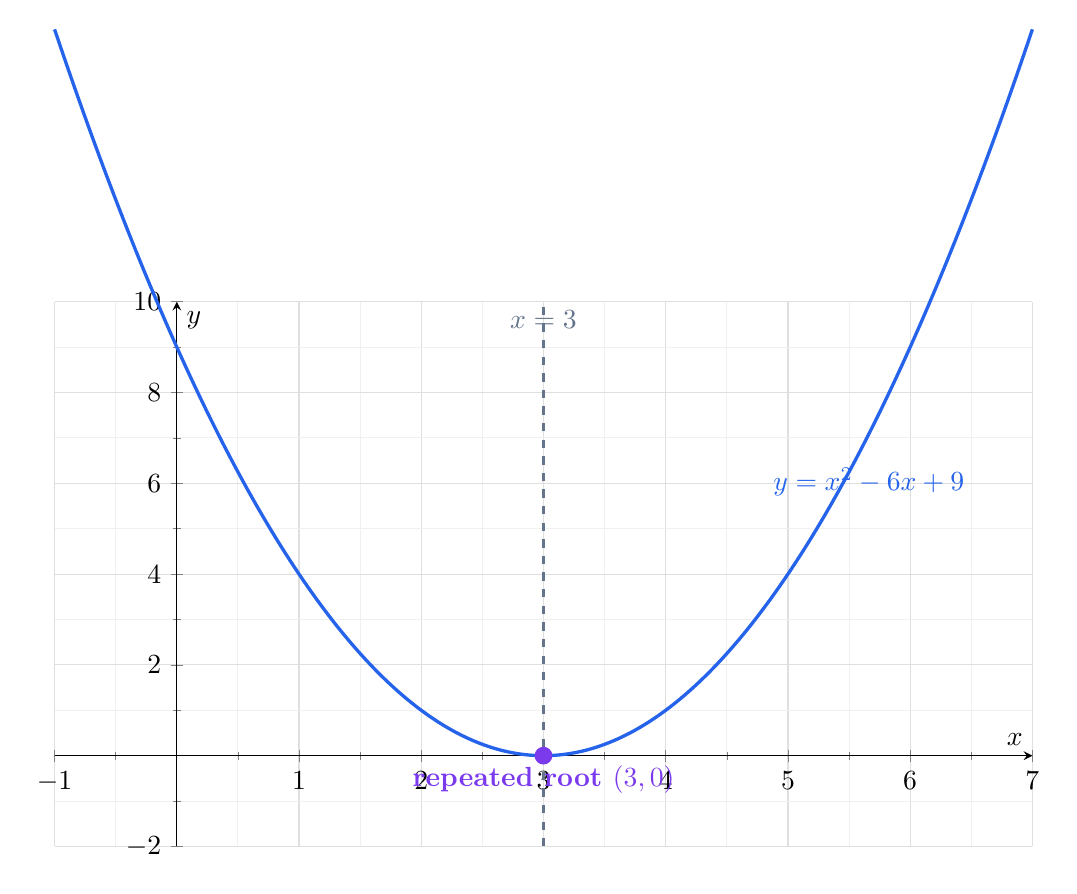
\begin{tikzpicture}
\begin{axis}[
width=14cm,height=8.5cm,
axis lines=middle,
xlabel={$x$},ylabel={$y$},
xmin=-1,xmax=7,ymin=-2,ymax=10,
grid=both,minor tick num=1,
major grid style={draw=gray!25},
minor grid style={draw=gray!12},
samples=240,
clip=false
]
\addplot[blue,very thick,domain=-1:7]{x^2-6*x+9};
\addplot[grayx,dashed,thick] coordinates {(3,-2)(3,10)};
\addplot[violet,only marks,mark=*,mark size=3pt] coordinates {(3,0)};
\node[anchor=south west,text=blue,font=\bfseries] at (axis cs:4.8,5.5){$y=x^2-6x+9$};
\node[anchor=south,text=grayx,font=\bfseries] at (axis cs:3,9.2){$x=3$};
\node[anchor=north,text=violet,font=\bfseries] at (axis cs:3,0){repeated root $(3,0)$};
\end{axis}
\end{tikzpicture}
\end{document}
